% !TeX root = ../thuthesis-example.tex

\chapter{系统测试与服务验收}

\section{接口自动化测试与 Newman 验证}



\begin{figure}[htbp]
  \centering
  
\includegraphics[width=0.9\textwidth,keepaspectratio]{figures/S11-newman-cli-real.png}
  \caption{Newman微服务接口测试报告}
  \label{fig:S11}
\end{figure}

为确保微服务对外提供的 RESTful 接口具备基本的鲁棒性与一致性，项目在开发交付阶段将 Apifox 导出的 Postman Collection 纳入 Newman 命令行回归验证。当前测试集合聚焦答辩现场最容易出现问题的网关认证与核心业务查询链路，覆盖验证码拉取、管理员登录、分类列表查询和订单分页查询四个接口，并在真实本地服务环境下执行断言。

系统测试集基于 Apifox 进行统一设计并导出为符合 Postman Collection v2.1 规范的 JSON 文件。网关代理测试部分包含通过 8090 端口发起的登录认证请求和验证码拉取请求，用于验证 Gateway 的外部入口、认证链路和跨域处理是否正常工作。登录认证测试用例向 /login 端点发送 POST 请求，请求体中包含用户名、密码、验证码和 uuid 字段，断言脚本检查响应状态码是否为 200、响应体 code 字段是否为成功标识 200，并提取响应中的 token 字段写入 Collection 变量以供后续接口复用。验证码拉取测试则向 /captchaImage 端点发送 GET 请求，断言响应中包含 captchaEnabled 字段并返回成功 code。由于当前运行验证环境已关闭验证码校验，测试脚本不再错误地要求 uuid 和 img 字段必须存在，避免把环境配置差异误判为接口失败。

业务端测试直连 lgg-business 的 8088 端口，覆盖分类列表查询和订单分页查询两个高频后台接口。分类查询断言响应 code 为 1 且 data 为非空数组，说明基础分类数据已经完成初始化并可被后台和小程序读取。订单查询断言响应 code 为 1 且 data.records 为数组，说明订单管理页面依赖的分页接口能够返回标准分页结构。上述接口均携带运行验证环境内部授权头，用于绕开浏览器会话状态对命令行测试造成的干扰，使 Newman 测试边界集中在服务可用性、响应结构和业务数据可读性上。



\begin{table}[htbp]
  \centering
  \caption{核心接口自动化回归测试用例表}
  \label{tab:api_tests}
  {\small
    \setlength{\tabcolsep}{4pt}%
    \begin{tabular}{>{\raggedright\arraybackslash}p{0.10\textwidth}>{\raggedright\arraybackslash}p{0.30\textwidth}>{\raggedright\arraybackslash}p{0.17\textwidth}>{\raggedright\arraybackslash}p{0.33\textwidth}}
    \toprule
    接口名称 & 请求路径 & 验证目标 & 核心断言规则 \\
    \midrule
    拉取验证码 & /captchaImage & 网关外部入口连通性 & 状态码 200，包含 captchaEnabled \\
    管理员登录 & /login & 认证拦截与令牌颁发 & 业务 code=200，返回有效 token \\
    分类列表查询 & /admin/category/list & 业务服务与缓存读取 & data 数组非空，响应耗时 <2s \\
    订单分页查询 & /admin/order/conditionSearch & 分页结构与跨服务查询 & data.records 非空，格式符合标准 \\
    \bottomrule
  \end{tabular}}
\end{table}

测试集中每个请求的 Tests 脚本标签页内编写了多维度的 JavaScript 自动断言。第一层断言统一检查 HTTP 响应状态码是否为 200，若非 200 则立即标记该用例为失败。第二层断言解析响应 JSON 体并检查业务操作成功标识字段 code 的值是否为预期的 200。第三层断言针对特定接口检查关键业务字段的存在性与格式正确性，例如登录接口必须返回非空的 token 字段，订单提交接口必须返回符合正则模式的业务订单号。第四层断言通过 pm.expect(responseTime).to.be.below(2000) 语句限制每个接口的响应时间不得超过 2000 毫秒，确保微服务在本地运行环境下的基本性能达标。

开发者在本地执行 npx newman run tests/apifox-collection.json --reporters cli 命令运行接口测试。Newman 的 CLI Reporter 在终端实时输出每个请求的执行状态和断言结果。本次截图所示运行结果中，请求总数为 4，断言总数为 8，失败数为 0，平均响应时间约为 70ms，说明网关认证入口与核心业务查询接口均能够在本地微服务环境下稳定响应。后续若继续扩展 Apifox 集合，可在同一命令入口下追加水果、套餐、购物车、支付回调和小票导出等更多业务场景。

\section{Playwright 核心闭环端到端（E2E）测试}



\begin{figure}[htbp]
  \centering
  
\includegraphics[width=0.9\textwidth,keepaspectratio]{figures/S12-playwright-cli-real.png}
  \caption{Playwright端到端闭环测试结果}
  \label{fig:S12}
\end{figure}

针对复杂的微服务协同场景，传统的接口测试难以覆盖跨服务的数据流转完整性，特别是从支付服务经过消息队列到通知服务再到浏览器前端 WebSocket 的全链路。为此本人使用微软开源的 Playwright 框架编写了端到端自动化测试用例，从真实浏览器的视角验证整个分布式系统的协同正确性。

测试架构设计遵循了测试金字塔理论中端到端测试层的设计原则。测试运行的前提条件要求全部微服务（lgg-admin, lgg-business, lgg-pay, lgg-notice, lgg-gateway）以及中间件（Redis, Nacos, MySQL, RabbitMQ）均已通过 PM2 正常启动，前端预览服务运行在固定的 8087 端口。测试配置文件 playwright.config.ts 中设置了 use.baseURL 为 http://127.0.0.1:8087，timeout 超时为 30000 毫秒，并指定使用 Chromium 浏览器引擎以 headless 无头模式运行，以提高测试执行速度和 CI 环境兼容性。

在测试数据初始化阶段，脚本在 beforeAll 钩子中自动建立 MySQL 数据库直连，使用 mysql2 驱动创建连接池并执行 SQL INSERT 语句向订单表直接插入一条状态为待付款的测试订单记录。该订单的业务订单号以 ORDER 前缀加时间戳命名以确保唯一性，购买用户设置为测试账户，实付金额设置为固定的测试值。通过 SQL 直接插入而非通过前端 UI 加购下单的设计意图是将测试边界锁定在支付至通知的核心微服务协同链路上，避免前端 UI 交互的不确定性对测试结果产生干扰。

测试执行流程包含五个关键步骤。第一步是 Token 注入绕过登录。传统的 UI 自动化登录需要处理验证码图片识别、密码输入以及页面跳转等待等复杂交互，在 CI 环境中极不稳定。因此 Playwright 测试采用 API 直接登录方案，脚本通过 page.request.post 方法向 Gateway 的 /auth/login 接口发送登录请求，请求体中包含预设的测试用户名和密码。获取响应中的 token 后，通过 page.context().addCookies 方法将 Admin-Token Cookie 注入到当前浏览器上下文中，随后调用 page.goto 方法直接导航至管理后台首页，完全绕过了登录页面的渲染与交互流程。这一技术权衡在保证测试覆盖了身份认证链路有效性的同时，大幅提升了测试执行的速度与稳定性。

第二步是前端页面访问验证。脚本导航至后台首页后通过 page.waitForSelector 等待核心 DOM 元素渲染完成，并通过 expect(page).toHaveTitle 断言页面标题包含生鲜关键字，确认前端应用已正常加载且 Token Cookie 认证有效。第三步是 WebSocket 消息订阅。脚本使用 Node.js 原生的 WebSocket 客户端直连通知微服务的 WebSocket 端点 ws://127.0.0.1:8086/ws/order，注册 onmessage 事件处理器并创建一个 Promise 用于异步等待消息到达。第四步是支付触发。脚本通过 page.request.post 方法直连支付微服务的 /pay/mock 接口发送 POST 请求，请求体中携带此前 SQL 插入的测试订单号和支付金额。第五步是消息断言与数据库验证。脚本通过 await 等待此前创建的 WebSocket Promise 在 15 秒超时内解析，断言收到的消息帧包含测试订单号以及"您有新的生鲜订单"提示语。随后脚本再次连接 MySQL 执行 SELECT 查询，读取该测试订单的当前状态字段值并断言其已变更为 2（表示已支付待接单），从底层数据库层面验证了 OpenFeign 远程调用确实成功修改了订单状态。

为了展示方便，系统在若依框架的密码校验服务中为 admin 用户添加了快捷放行逻辑，该放行仅作为本地开发与测试环境快速打通身份认证的临时举措，并非生产级安全设计，在正式部署时应当移除。全部端到端测试用例在本地运行后以 100\% 的通过率完成，Playwright 自动生成的 HTML 测试报告详细记录了每个测试步骤的执行时间和断言结果。

\section{微服务健康监控与全局看板}
\begin{figure}[htbp]
  \centering
  
\includegraphics[width=0.9\textwidth,keepaspectratio]{figures/S02-nacos-services-real.png}
  \caption{Nacos服务注册中心}
  \label{fig:S02}
\end{figure}

\begin{figure}[htbp]
  \centering
  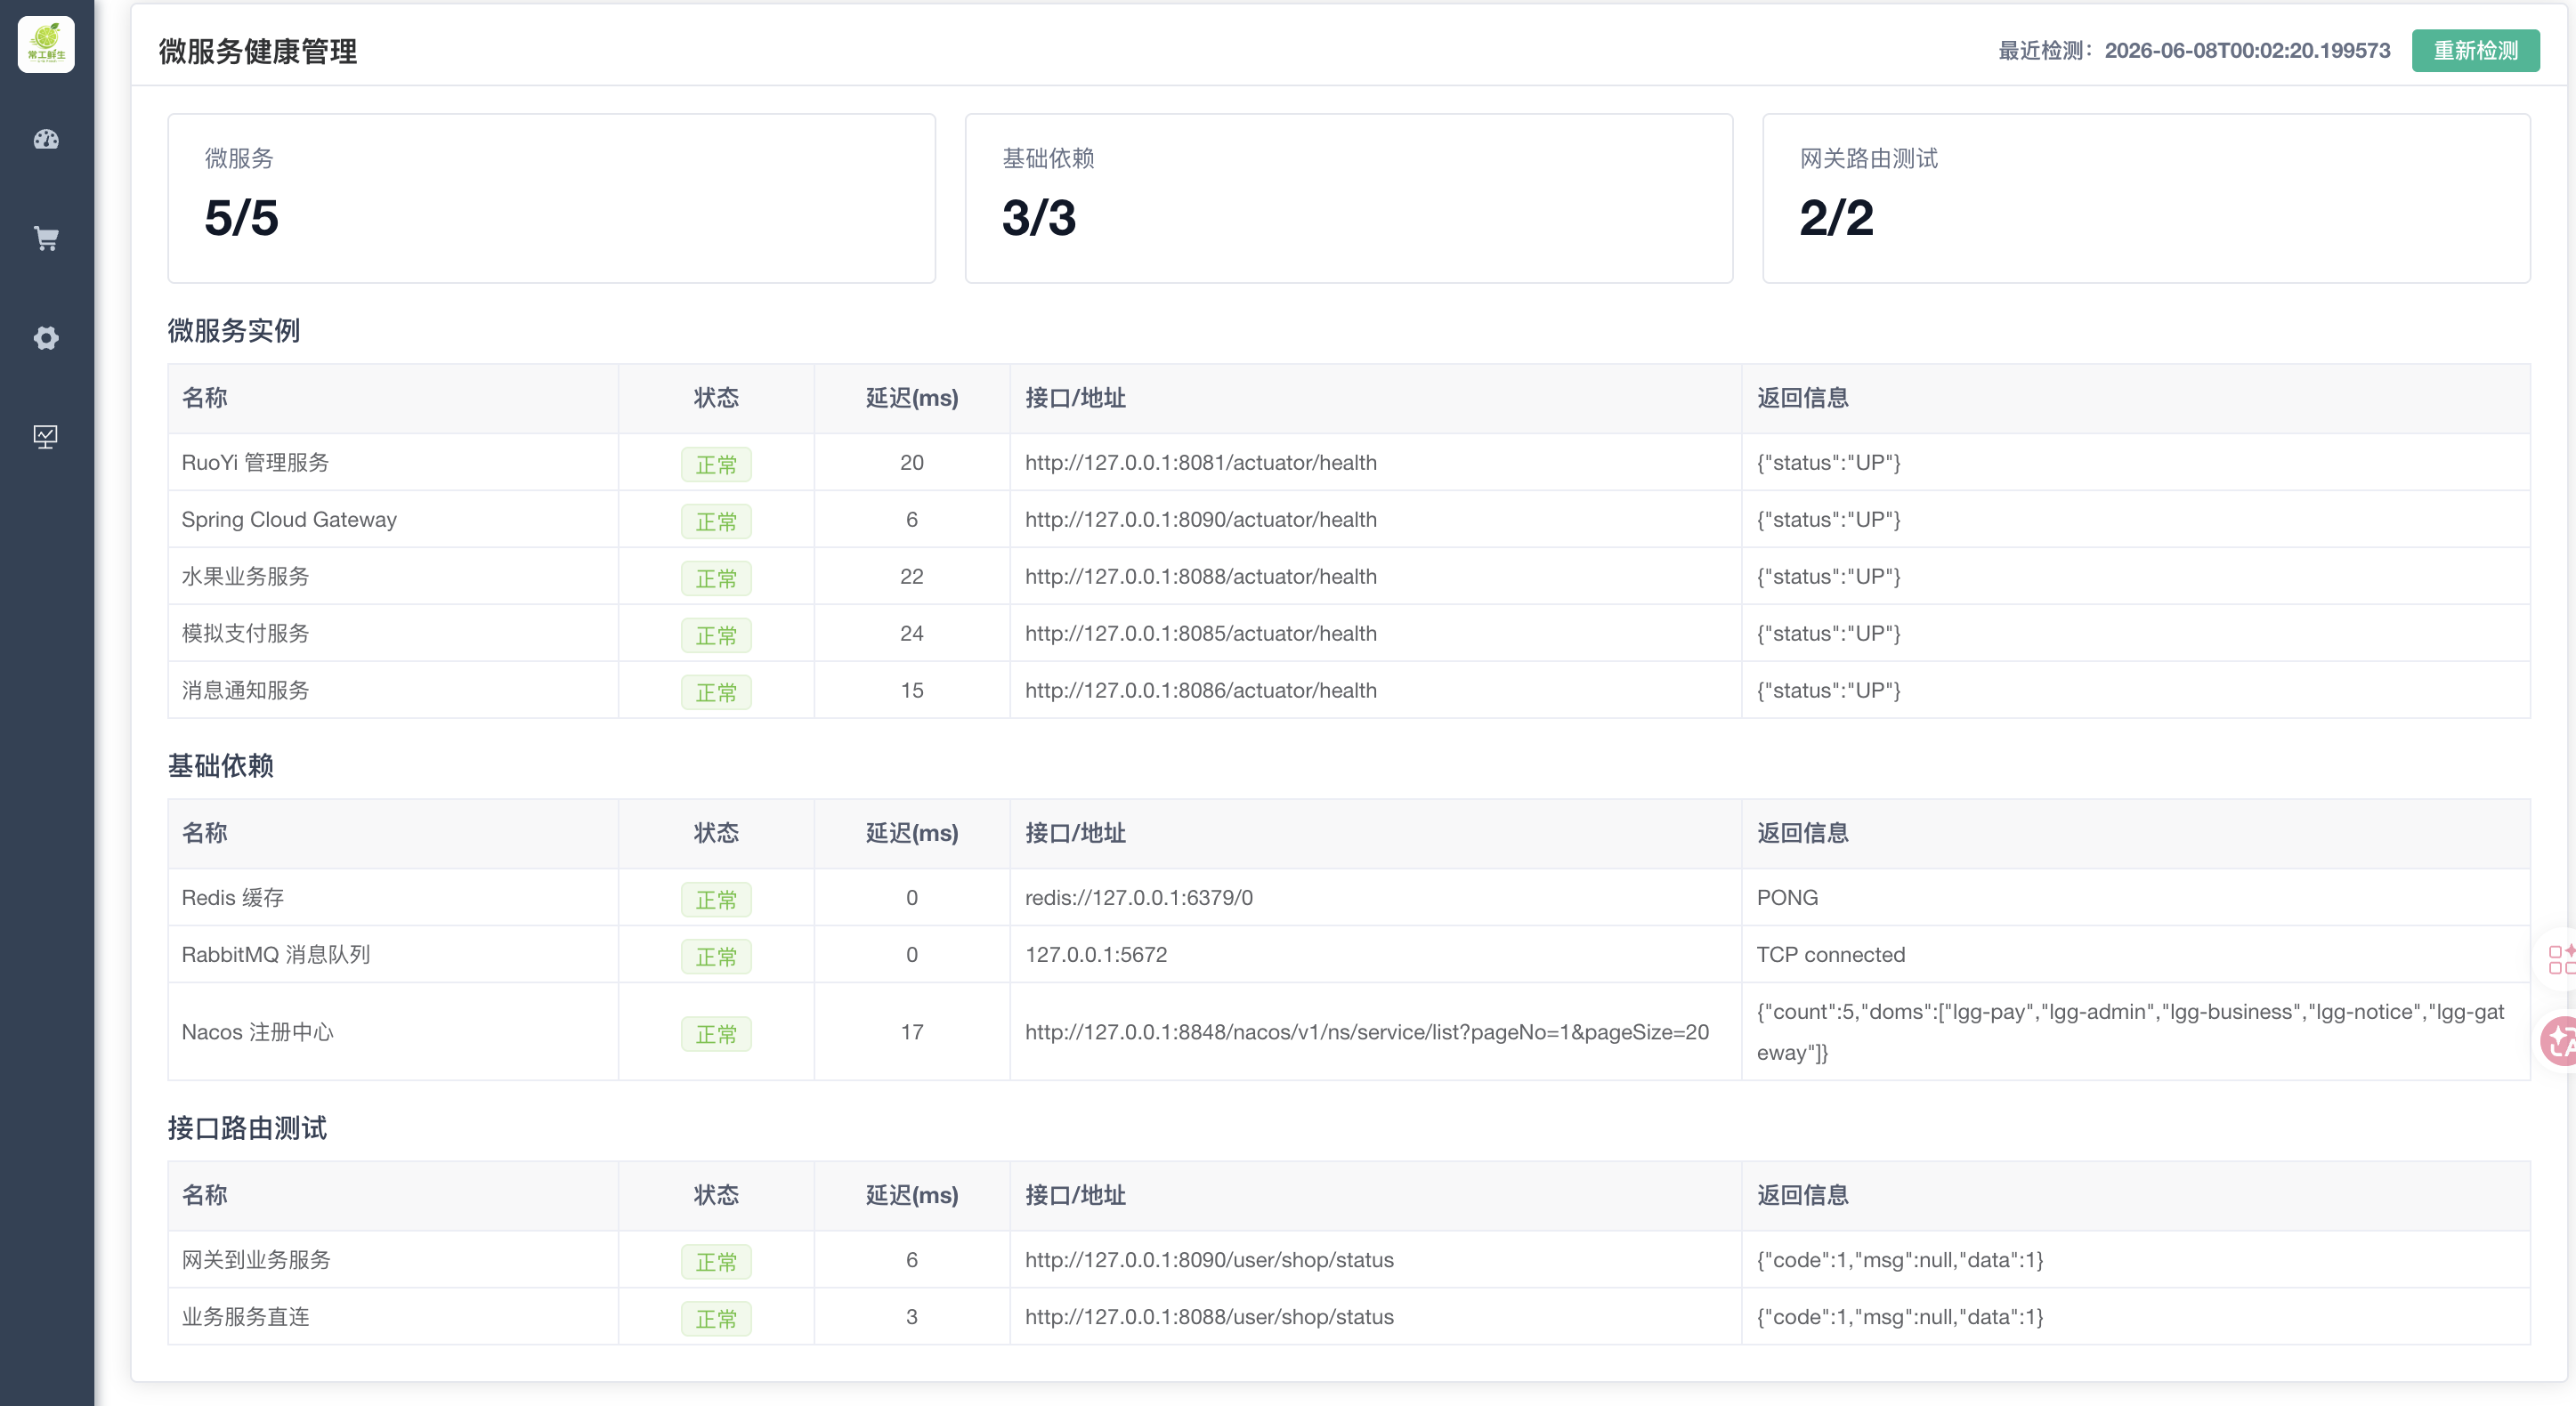
\includegraphics[width=0.9\textwidth,keepaspectratio]{figures/S06-health-dashboard.png}
  \caption{微服务健康监控与全局看板}
  \label{fig:health}
\end{figure}


在微服务架构中，由于各个服务分布在不同的进程与端口中，统一的健康监控面板对于系统运维至关重要。如上图 \ref{fig:health} 所示，系统实现了一个全局微服务健康看板，用于对核心服务及其基础依赖的存活状态进行实时遥测。该看板主要分为三个维度的检测：

首先是微服务实例本身的状态监测（图左侧 5/5 在线）。各个微服务集成了 `spring-boot-starter-actuator` 运行时监控组件，并通过 `management.endpoints.web.exposure.include=health` 将健康端点开放给外部。监控大屏通过 Gateway 网关依次调用 `lgg-admin`、`lgg-gateway`、`lgg-business`、`lgg-pay` 和 `lgg-notice` 的 `/actuator/health` 接口，并解析其返回的 `{"status":"UP"}` 数据，展示当前延迟（通常在 6ms~24ms 之间），确保微服务进程自身能够正常响应 HTTP 请求。

其次是基础中间件依赖的连通性监控（图中部 3/3 正常）。在分布式环境中，即使微服务进程正常运行，如果底层的数据库或消息队列中断，业务同样会瘫痪。由于各微服务内部配置了 Redis、RabbitMQ 和 Nacos 的连接，Actuator 会利用内置的 `RedisHealthIndicator`、`RabbitHealthIndicator` 自动发送 PING 心跳指令并捕获 PONG 回复。监控面板汇总这些信息，直观地证明了从应用到中间件的 TCP 长连接处于健康可用状态。

最后是网关路由与直连测试的比对（图右侧 2/2 正常）。面板对同一个核心业务端点 `/user/shop/status` 发起了两次并行探测，一次通过 `http://127.0.0.1:8090/...` 走网关转发，另一次通过 `http://127.0.0.1:8088/...` 绕过网关直连。通过比对两者的返回信息（`{"code":1,"data":1}`）与延迟差距，可以验证 Gateway 的动态路由功能工作正常且未引入过高的性能损耗。



每个微服务在开发阶段均引入了 spring-boot-starter-actuator 运行时监控组件。Actuator 通过 Spring Boot 的条件自动装配机制在应用启动时自动注册一系列管理端点。项目在各微服务的 application.yml 配置文件中通过 management.endpoints.web.exposure.include 属性显式暴露了 health 健康检查端点，确保外部监控系统能够通过 HTTP GET 请求访问该端点获取服务运行状态。对于支付和通知微服务，由于它们在启动类中排除了 Spring Security 的自动配置，因此健康端点无需额外的安全放行配置即可被外部直接访问。对于管理服务 lgg-admin，则在其安全配置类 SecurityConfig 中将 /actuator/所有子路径 添加至白名单以允许匿名访问。

当外部系统对某个微服务的 /actuator/health 端点发起 GET 请求时，Actuator 内置的健康指示器会自动执行一系列组件级别的连通性探测。对于包含数据源配置的微服务，DataSourceHealthIndicator 会向底层 MySQL 数据库发送一条 SELECT 1 验证查询以确认物理连接的可用性。对于集成了 Redis 的微服务，RedisHealthIndicator 会执行 PING 命令并检查是否收到 PONG 响应。DiskSpaceHealthIndicator 则检测当前工作目录所在磁盘分区的剩余空间是否超过配置的阈值（默认为 10MB）。所有指示器的检测结果汇总后，若全部组件均处于可用状态，则端点返回包含 status 字段值为 UP 的 JSON 响应体；若任一组件检测失败，则 status 变更为 DOWN 并附带故障组件的详细错误信息。

通过 Gateway 网关的路由规则，运维人员可以使用统一的网关入口地址代理访问各个微服务的健康端点，而无需记忆每个服务的独立端口。例如通过 http://127.0.0.1:8090/system/actuator/health 可路由至 lgg-admin 的健康端点，通过 http://127.0.0.1:8090/business/actuator/health 可路由至 lgg-business 的健康端点。在 Nacos 注册中心的管理控制台中，每个已注册的微服务实例旁边均展示 Healthy Instance Count 健康实例计数，当该计数值为 1 时表示当前有一个健康实例正在运行且持续通过 Nacos 的心跳检测。运维人员通过网关的健康监控以及 Nacos 注册中心控制台的综合视图，可以第一视角确定当前运行中的各微服务实例均处于健康治理状态下，及时发现并处置潜在的服务异常。
